\label{chap.7}
\section{Allocation Problem}
\label{sec:allocation_problem}
The last learned component shares the capacity of each cell between the eMBB, URLLC and mMTC slices. Every cell has its own agent. The agent sees 17 local quantities: the demand, utilisation and QoS of each slice, its previous allocation, the time of day, and the forecast when one is given. It outputs four non-negative numbers, and a softmax turns them into the shares of eMBB, URLLC, mMTC and idle capacity. The environment of Chapter~\ref{chap.4} then works out the QoS, the SLA outcomes and the reward. The cells affect each other only through interference, since the usable capacity of a cell drops when its neighbours are loaded.

\section{Scalable MARL Design}
\label{sec:scalable_marl}
All cells share one actor, a network with 19{,}332 parameters that maps the observation of a cell to its allocation. The actor never looks at other cells, so the same copy works at any network size. Training uses a centralised critic that looks at the neighbourhood: it takes the observation and action of a cell together with the mean observation and mean action of its grid neighbours. The reward of each agent also contains a share of its neighbours' rewards, which pushes the agents to coordinate locally.

The learning algorithm is an actor--critic in the style of MADDPG \cite{lowe2017}. It uses a replay buffer of 50{,}000 transitions, a discount factor of 0.9, soft target updates with $\tau=0.01$, learning rates of $3\times10^{-4}$ for the actor and $10^{-3}$ for the critic, and exploration noise added in logit space. The earlier B5G trainer used the observed reward as a one-step target, because its offline samples are single decisions and not interactions with a simulator.

\section{Evaluation Protocol}
\label{sec:marl_protocol}
Every result in this chapter uses the same protocol. Agents train on days 1 to 40 of the recorded data. Days 41 to 44 are only used to pick a checkpoint or tune a rule. The test is the held-out week of 16 to 22 December 2013, with one reward per day, and each table entry is the mean of those seven days. We compare two controllers day by day and quote a 95\% interval on the mean difference, using a $t$ value for six degrees of freedom. Consecutive days are not independent, so the intervals only describe how much the days of this one week vary; they say nothing about another week or another city. Learned policies are also averaged over several seeds, and every table gives the number of seeds.

\section{MARL versus a Single Central Agent}
\label{sec:marl_comparison}
The first question is whether splitting the problem into local agents matters. A single central agent sees the observations of all cells and outputs all the allocations at once. We trained it with two learning rates, on the same data, reward and number of episodes. Table~\ref{tab:marl_scaling} shows the result at a budget of 1{,}000 episodes.

\begin{table}[htbp]
\centering
\caption{Held-out week reward at a training budget of 1{,}000 episodes (mean over seeds, number of seeds in brackets)}
\label{tab:marl_scaling}
\footnotesize
\begin{tabular}{|>{\centering\arraybackslash}p{\dimexpr 0.121\textwidth-2\tabcolsep\relax}|>{\centering\arraybackslash}p{\dimexpr 0.121\textwidth-2\tabcolsep\relax}|>{\centering\arraybackslash}p{\dimexpr 0.121\textwidth-2\tabcolsep\relax}|>{\centering\arraybackslash}p{\dimexpr 0.121\textwidth-2\tabcolsep\relax}|>{\centering\arraybackslash}p{\dimexpr 0.121\textwidth-2\tabcolsep\relax}|>{\centering\arraybackslash}p{\dimexpr 0.121\textwidth-2\tabcolsep\relax}|>{\centering\arraybackslash}p{\dimexpr 0.121\textwidth-2\tabcolsep\relax}|>{\centering\arraybackslash}p{\dimexpr 0.121\textwidth-2\tabcolsep\relax}|}
\hline
\textbf{Cells} & \textbf{Shared MARL} & \textbf{Single agent (lr $10^{-4}$ / $3\times10^{-4}$)} & \textbf{Equal split} & \textbf{Expert, current} & \textbf{Expert, forecast} & \textbf{Expert, forecast, tuned} & \textbf{Expert, true next} \\ \hline
9 & $0.926\pm0.005$ (2) & 0.433 / 0.442 & 0.785 & 0.794 & 0.825 & 0.909 & 0.945 \\ \hline
25 & $0.833\pm0.086$ (2) & 0.337 / 0.329 & 0.750 & 0.775 & 0.804 & 0.877 & 0.920 \\ \hline
100 & 0.857 (1) & 0.284 / 0.267 & 0.735 & 0.765 & 0.794 & 0.865 & 0.908 \\ \hline
\end{tabular}
\end{table}

\begin{figure}[htbp]
\centering
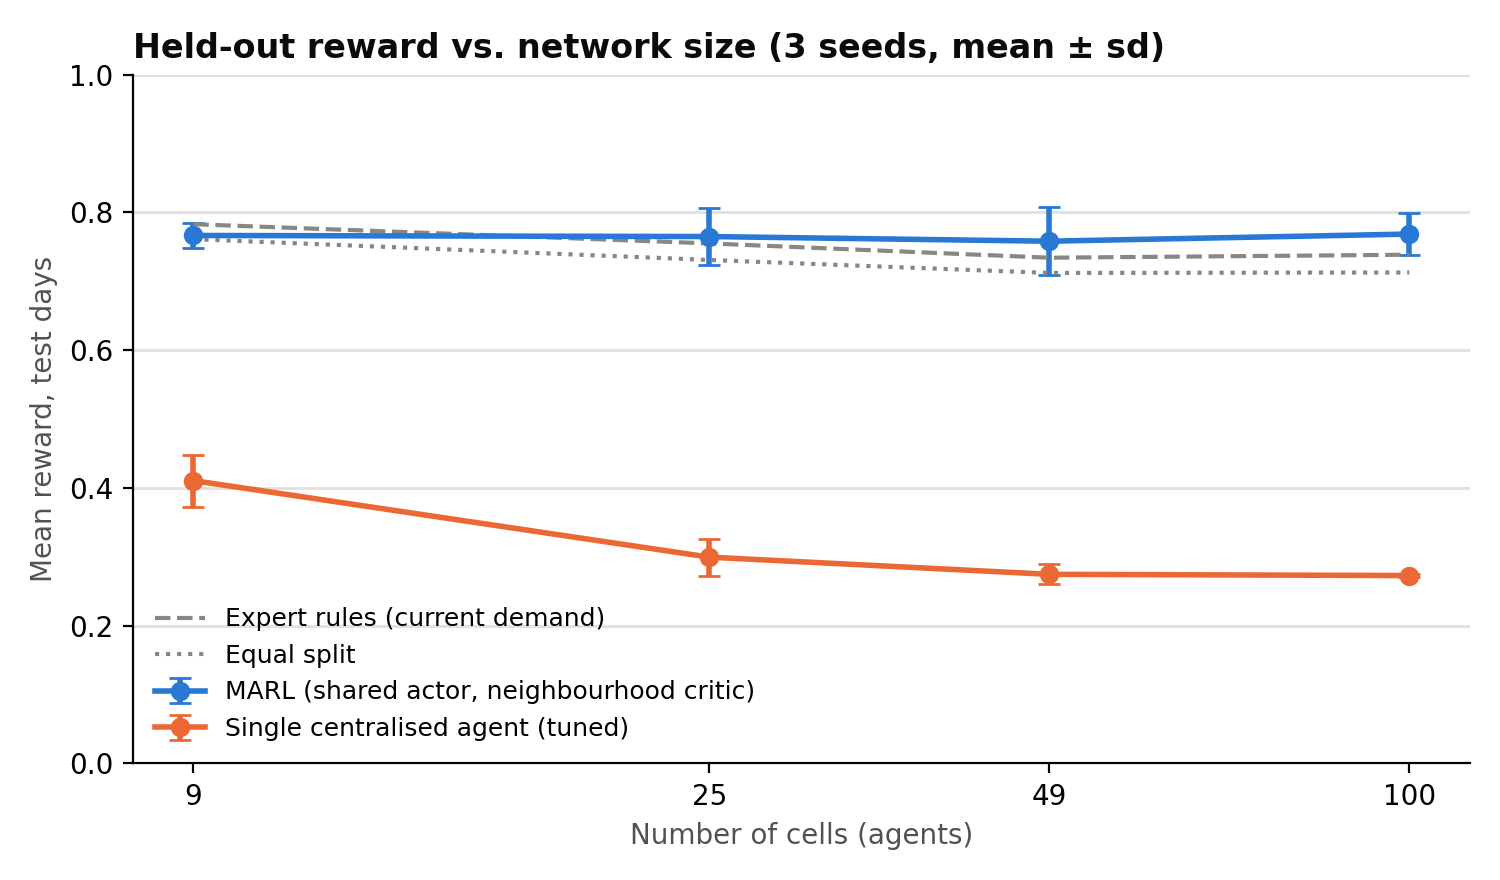
\includegraphics[width=0.85\textwidth,keepaspectratio]{unified_marl_vs_single.png}
\caption{Reward against network size: shared MARL, the single agent and the reference rules}
\label{fig:marl_scaling}
\end{figure}

The shared actor keeps both its size and its reward as the network grows. The central actor, in contrast, grows from 114{,}468 to 604{,}048 parameters (Table~\ref{tab:marl_parameter_growth}) and its reward falls from about 0.43 to 0.27--0.28. This supports the split into local agents. The central agent has to learn a very large action space from one learning step per episode step, and in our runs its reward went down during training instead of up. So the result tells us that this central baseline works badly, not that every centralised design would. Sharing parameters is the natural way to keep the problem manageable, and that is the point of the comparison.

\begin{table}[htbp]
\centering
\caption{Policy size as the network grows}
\label{tab:marl_parameter_growth}
\footnotesize
\begin{tabular}{|>{\centering\arraybackslash}p{\dimexpr 0.300\textwidth-2\tabcolsep\relax}|>{\centering\arraybackslash}p{\dimexpr 0.170\textwidth-2\tabcolsep\relax}|>{\centering\arraybackslash}p{\dimexpr 0.170\textwidth-2\tabcolsep\relax}|>{\centering\arraybackslash}p{\dimexpr 0.170\textwidth-2\tabcolsep\relax}|}
\hline
\textbf{Cells} & \textbf{Shared actor parameters} & \textbf{Single-agent actor parameters} & \textbf{Central input / output size} \\ \hline
9 & 19{,}332 & 114{,}468 & 153 / 36 \\ \hline
25 & 19{,}332 & 200{,}548 & 425 / 100 \\ \hline
100 & 19{,}332 & 604{,}048 & 1700 / 400 \\ \hline
\end{tabular}
\end{table}

\section{Comparison with Properly Tuned Rules}
\label{sec:marl_vs_tuned}
A learned controller should also be compared with the strongest simple one, not only with an equal split. The expert rule gives URLLC and mMTC enough capacity to hold their utilisation at a target, and the rest to eMBB. Its default targets were picked by hand, so we built two tuned versions that use the training days only.
\begin{itemize}
\item \textbf{Simple tuned rule.} Two utilisation targets, one for URLLC and one for mMTC, are chosen by grid search on the training days. At 25 cells the search picks 0.4 and 0.4, and the held-out reward of the forecast-fed rule rises from 0.804 to 0.878.
\item \textbf{Rich tuned rule.} The targets are chosen separately for each four-hour block of the day and each of three cell classes (by traffic level), 18 pairs in total.
\end{itemize}
Table~\ref{tab:marl_scaling} shows that at 1{,}000 episodes the shared MARL controller is clearly better than the untuned rules, but at 25 and 100 cells it loses to the simple tuned rule. We therefore moved to a longer protocol: 4{,}000 episodes, the checkpoint with the best validation reward, and an average of the actors from several seeds in logit space. Table~\ref{tab:marl_long} gives the result.

\begin{table}[htbp]
\centering
\caption{Long protocol (4{,}000 episodes, checkpoint chosen on validation days, actors averaged in logit space) against the tuned expert rules, held-out week (difference in reward, 95\% CI, days better out of 7)}
\label{tab:marl_long}
\footnotesize
\begin{tabular}{|>{\centering\arraybackslash}p{\dimexpr 0.139\textwidth-2\tabcolsep\relax}|>{\centering\arraybackslash}p{\dimexpr 0.139\textwidth-2\tabcolsep\relax}|>{\centering\arraybackslash}p{\dimexpr 0.139\textwidth-2\tabcolsep\relax}|>{\centering\arraybackslash}p{\dimexpr 0.139\textwidth-2\tabcolsep\relax}|>{\centering\arraybackslash}p{\dimexpr 0.139\textwidth-2\tabcolsep\relax}|>{\centering\arraybackslash}p{\dimexpr 0.139\textwidth-2\tabcolsep\relax}|>{\centering\arraybackslash}p{\dimexpr 0.139\textwidth-2\tabcolsep\relax}|}
\hline
\textbf{Cells} & \textbf{MARL (actors)} & \textbf{Simple tuned expert} & \textbf{MARL minus simple} & \textbf{Rich tuned expert} & \textbf{MARL minus rich} & \textbf{True-next oracle} \\ \hline
9 & 0.933 (3) & 0.909 & +0.024 $\pm$ 0.004 (7/7) & 0.928 & +0.005 $\pm$ 0.004 (6/7) & 0.945 \\ \hline
25 & 0.904 (3) & 0.877 & +0.026 $\pm$ 0.005 (7/7) & 0.899 & +0.005 $\pm$ 0.003 (7/7) & 0.920 \\ \hline
100 & 0.888 (1) & 0.865 & +0.023 $\pm$ 0.006 (7/7) & 0.887 & +0.001 $\pm$ 0.003 (3/7) & 0.908 \\ \hline
\end{tabular}
\end{table}

\begin{figure}[htbp]
\centering
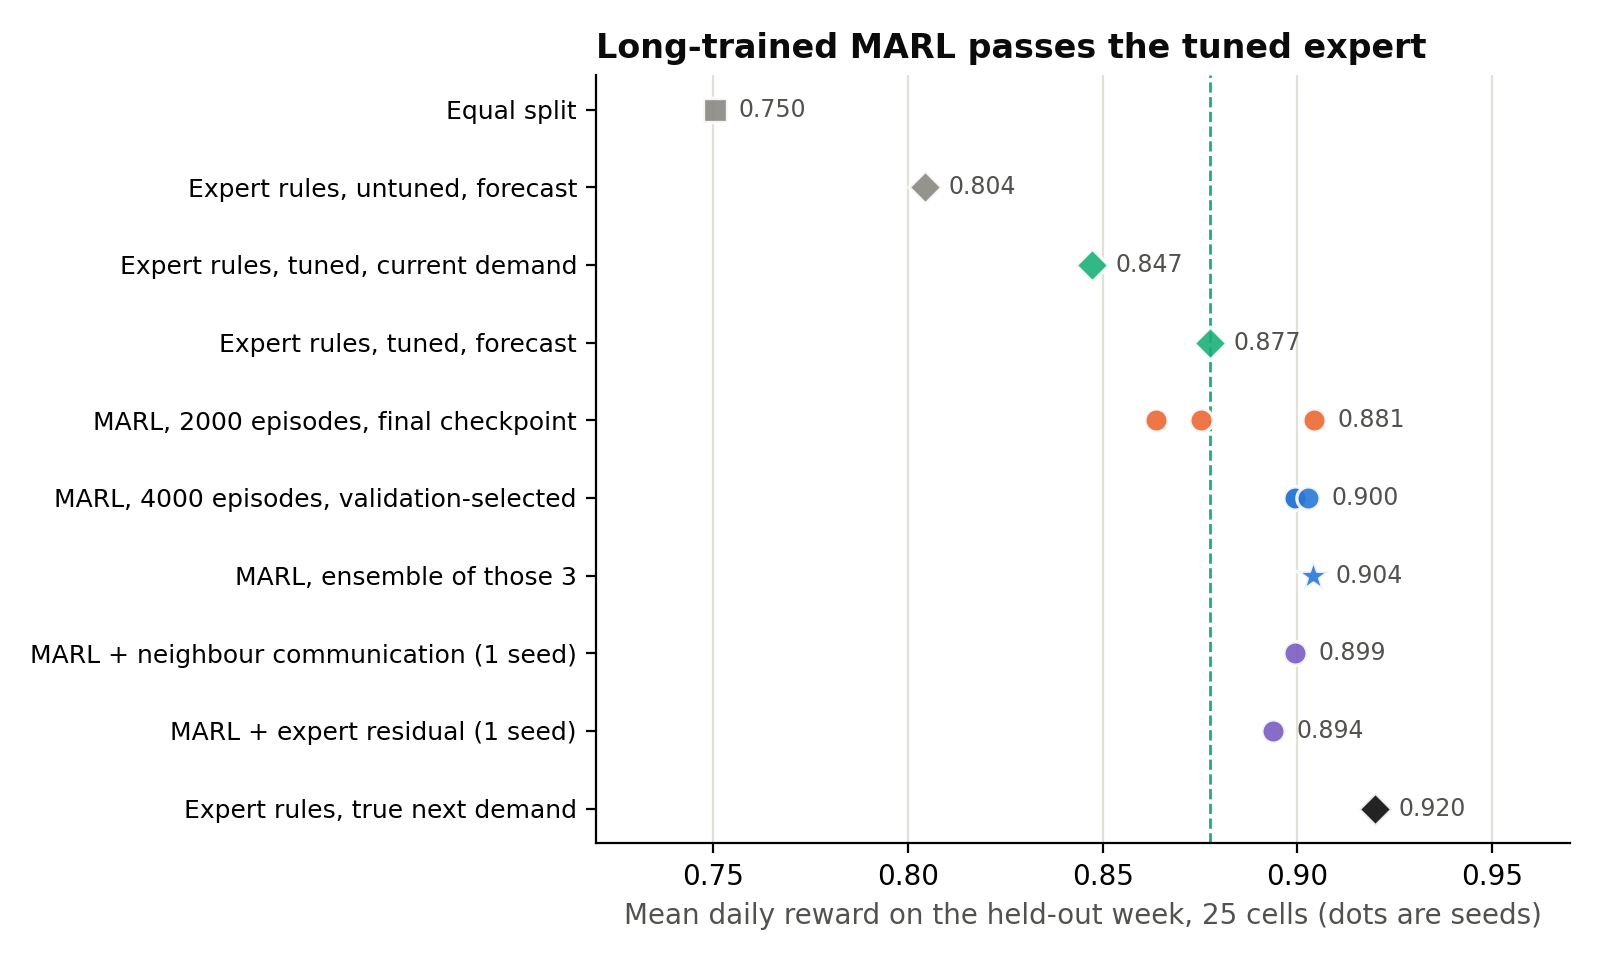
\includegraphics[width=0.9\textwidth,keepaspectratio]{unified_marl_best.png}
\caption{Long-protocol MARL against the tuned rules on the held-out week}
\label{fig:marl_best}
\end{figure}

Against the simple tuned rule, the learned controller is better on each of the seven test days at 9, 25 and 100 cells, by 0.023 to 0.024 in reward. Against the rich tuned rule the difference is about 0.005 or less, and at 25 and 100 cells the intervals include zero. So the off-policy controller matches a carefully tuned rule that knows the time of day and beats a simply tuned one, but it does not clearly beat the strongest hand-built rule. The on-policy learners of Section~\ref{sec:marl_ppo} do go beyond it. The 100-cell result rests on one seed, and its interval only describes the seven days.

\subsection{What the learned controller does}
Table~\ref{tab:marl_diagnosis} compares the allocations. The learned controller gives URLLC and mMTC about twice the capacity that the untuned rule gives them (shares of 0.23 and 0.09 against 0.11 and 0.04), so their SLAs are almost always met. It accepts a slightly lower share of eMBB demand served, and overall the reward is higher. This is a sensible policy and not an accident of the numbers, and the tuned rule ends up in the same place.

\begin{table}[htbp]
\centering
\caption{What the learned controller does differently (25 cells, held-out week; SLA rates, fraction of demand served, and mean capacity share per slice)}
\label{tab:marl_diagnosis}
\footnotesize
\begin{tabular}{|>{\centering\arraybackslash}p{\dimexpr 0.194\textwidth-2\tabcolsep\relax}|>{\centering\arraybackslash}p{\dimexpr 0.194\textwidth-2\tabcolsep\relax}|>{\centering\arraybackslash}p{\dimexpr 0.194\textwidth-2\tabcolsep\relax}|>{\centering\arraybackslash}p{\dimexpr 0.194\textwidth-2\tabcolsep\relax}|>{\centering\arraybackslash}p{\dimexpr 0.194\textwidth-2\tabcolsep\relax}|}
\hline
\textbf{Controller} & \textbf{SLA met (eMBB / URLLC / mMTC)} & \textbf{Demand served} & \textbf{Capacity share (eMBB / URLLC / mMTC)} & \textbf{Reward} \\ \hline
Shared MARL (2{,}000 episodes, seed 0) & 0.68 / 0.99 / 1.00 & 0.92 & 0.68 / 0.23 / 0.09 & 0.904 \\ \hline
Expert rule, forecast, untuned & 0.72 / 0.80 / 0.61 & 0.95 & 0.85 / 0.11 / 0.04 & 0.804 \\ \hline
Expert rule, true next demand & 0.72 / 1.00 / 1.00 & 0.95 & 0.85 / 0.11 / 0.04 & 0.920 \\ \hline
Equal split & 0.18 / 0.99 / 1.00 & 0.77 & 0.33 / 0.33 / 0.33 & 0.750 \\ \hline
\end{tabular}
\end{table}

\section{Training Variants}
\label{sec:marl_variants}
We tried several ways to improve the learner at 25 cells (Table~\ref{tab:marl_variants}): explicit communication between neighbouring actors, an expert-residual policy in which the actor outputs a correction to the allocation of the rule, a loss regularised towards the expert in the style of TD3+BC \cite{fujimoto2021minimalist}, and richer observations. None of them is clearly better than the plain shared actor trained with the long protocol and averaged. The on-policy learners of Section~\ref{sec:marl_ppo} are the exception. An actor with richer observations does not beat the rich tuned rule (a difference of $-0.007\pm0.009$, better on 2 of 7 days). The variants with one seed are only hints and should not be read as a ranking.

\begin{table}[htbp]
\centering
\caption{Training variants at 25 cells, held-out week reward}
\label{tab:marl_variants}
\footnotesize
\begin{tabular}{|>{\centering\arraybackslash}p{\dimexpr 0.300\textwidth-2\tabcolsep\relax}|>{\centering\arraybackslash}p{\dimexpr 0.170\textwidth-2\tabcolsep\relax}|>{\centering\arraybackslash}p{\dimexpr 0.170\textwidth-2\tabcolsep\relax}|}
\hline
\textbf{Variant} & \textbf{Seeds} & \textbf{Reward} \\ \hline
Shared DDPG, 2{,}000 episodes, with forecast & 3 & $0.881\pm0.021$ \\ \hline
Expert-regularised loss (TD3+BC style), no forecast & 3 & $0.844\pm0.065$ \\ \hline
Neighbour communication in the actor & 1 & 0.899 \\ \hline
Expert-residual policy & 1 & 0.894 \\ \hline
Communication and expert residual & 1 & 0.892 \\ \hline
Long protocol, ensemble of three actors & 3 & 0.904 \\ \hline
Long protocol with extra observations, ensemble & 2 & 0.892 \\ \hline
\end{tabular}
\end{table}

\section{On-Policy Baselines}
\label{sec:marl_ppo}
To compare with the off-policy design we also implemented independent PPO (IPPO) and a MAPPO-style variant \cite{schulman2017ppo, yu2022mappo, dewitt2020ippo}. The policy is a Gaussian over the four logits. Advantages come from generalised advantage estimation \cite{schulman2016gae} with $\lambda=0.95$ and $\gamma=0.9$ on the team reward, the clipping parameter is 0.2, and each update uses 10 episodes. In IPPO the actor and the value function of a cell only see that cell. In MAPPO the value function also sees the mean observation of the grid neighbours, which is the neighbourhood form of a centralised critic as in the DDPG critic, while the actor stays local. Both were trained for 8{,}000 episodes with the same checkpoint rule. Table~\ref{tab:marl_ppo} gives the outcome. All 12 runs end at almost the same reward, between 0.907 and 0.908, whichever variant or seed is used. This is higher than the off-policy controller of the previous sections (0.904) and higher than the rich tuned rule (0.899): averaged over the runs the difference to the rich rule is +0.009 $\pm$ 0.002, with a gain on 7 of 7 days, and every single run beats the rich rule on all seven days. The true-next-demand rule, which uses information no deployable controller has, is still higher at 0.920. IPPO and MAPPO give the same result, so in this environment the neighbourhood term in the value function brings no measurable benefit. The near-identical outcome of independent seeds suggests that the on-policy learner reliably finds the same good allocation behaviour, and that the remaining gap to the oracle comes from demand that cannot be predicted ten minutes ahead.

\begin{table}[htbp]
\centering
\caption{On-policy baselines at 25 cells (8{,}000 episodes, checkpoint chosen on validation days), held-out week}
\label{tab:marl_ppo}
\footnotesize
\begin{tabular}{|>{\centering\arraybackslash}p{\dimexpr 0.194\textwidth-2\tabcolsep\relax}|>{\centering\arraybackslash}p{\dimexpr 0.194\textwidth-2\tabcolsep\relax}|>{\centering\arraybackslash}p{\dimexpr 0.194\textwidth-2\tabcolsep\relax}|>{\centering\arraybackslash}p{\dimexpr 0.194\textwidth-2\tabcolsep\relax}|>{\centering\arraybackslash}p{\dimexpr 0.194\textwidth-2\tabcolsep\relax}|}
\hline
\textbf{Method} & \textbf{Seeds} & \textbf{Reward} & \textbf{Minus simple tuned expert} & \textbf{Minus rich tuned expert} \\ \hline
IPPO & 3 & $0.908\pm0.000$ & +0.030 & +0.009 \\ \hline
MAPPO & 9 & $0.908\pm0.000$ & +0.030 & +0.009 \\ \hline
Shared DDPG, long protocol, ensemble & 3 & 0.904 & +0.026 & +0.005 \\ \hline
\end{tabular}
\end{table}

\section{Robustness to Traffic Shifts}
\label{sec:marl_shift}
A controller trained on ordinary traffic may fail when the traffic changes. We therefore replayed the held-out week with the two scenario multipliers of Chapter~\ref{chap.8}, 6G growth and a massive-IoT surge. Table~\ref{tab:marl_shift} gives the results for controllers that were not retrained.

\begin{table}[htbp]
\centering
\caption{Controllers trained on ordinary traffic, run on shifted traffic (25 cells, held-out week, DDPG-MARL averaged over three 2{,}000-episode seeds)}
\label{tab:marl_shift}
\footnotesize
\begin{tabular}{|>{\centering\arraybackslash}p{\dimexpr 0.162\textwidth-2\tabcolsep\relax}|>{\centering\arraybackslash}p{\dimexpr 0.162\textwidth-2\tabcolsep\relax}|>{\centering\arraybackslash}p{\dimexpr 0.162\textwidth-2\tabcolsep\relax}|>{\centering\arraybackslash}p{\dimexpr 0.162\textwidth-2\tabcolsep\relax}|>{\centering\arraybackslash}p{\dimexpr 0.162\textwidth-2\tabcolsep\relax}|>{\centering\arraybackslash}p{\dimexpr 0.162\textwidth-2\tabcolsep\relax}|}
\hline
\textbf{Traffic} & \textbf{Equal split} & \textbf{Expert tuned on ordinary} & \textbf{Expert re-tuned on this traffic} & \textbf{MARL with forecast} & \textbf{MARL without forecast} \\ \hline
Ordinary traffic & 0.750 & 0.877 & 0.877 & 0.881 & 0.851 \\ \hline
6G growth (eMBB $\times$1.3, URLLC $\times$2, mMTC $\times$3) & 0.615 & 0.762 & 0.762 & 0.724 & 0.692 \\ \hline
Massive IoT (mMTC $\times$10) & 0.666 & 0.725 & 0.735 & 0.672 & 0.685 \\ \hline
\end{tabular}
\end{table}

When the traffic shifts, the learned controllers lose a lot of reward, and a rule that is re-tuned on the new traffic is clearly better. The forecast input helps the learned policy on ordinary traffic and under 6G growth (by about 0.03) and costs about 0.01 under the surge, so its effect is not consistent. Training on a mixture of scenarios solves the problem (Table~\ref{tab:marl_robust}). The policy trained on the mixture beats an expert re-tuned on the training days of each scenario in every traffic condition on average. The gain is clear on ordinary traffic and under 6G growth, and it is within noise under the massive-IoT surge.

\begin{table}[htbp]
\centering
\caption{MARL trained on a mixture of traffic scenarios (two seeds, actors averaged), against an expert rule re-tuned on each scenario's own training days}
\label{tab:marl_robust}
\footnotesize
\begin{tabular}{|>{\centering\arraybackslash}p{\dimexpr 0.300\textwidth-2\tabcolsep\relax}|>{\centering\arraybackslash}p{\dimexpr 0.170\textwidth-2\tabcolsep\relax}|>{\centering\arraybackslash}p{\dimexpr 0.170\textwidth-2\tabcolsep\relax}|>{\centering\arraybackslash}p{\dimexpr 0.170\textwidth-2\tabcolsep\relax}|}
\hline
\textbf{Test traffic} & \textbf{MARL reward} & \textbf{Difference (95\% CI)} & \textbf{Days better} \\ \hline
Ordinary traffic & 0.904 & +0.026 $\pm$ 0.003 & 7/7 \\ \hline
6G growth & 0.780 & +0.018 $\pm$ 0.002 & 7/7 \\ \hline
Massive IoT & 0.738 & +0.003 $\pm$ 0.003 & 6/7 \\ \hline
\end{tabular}
\end{table}

\section{Earlier B5G MADDPG Development}
\label{sec:b5g-maddpg}
Before the unified Milan environment existed, we implemented MADDPG on the B5G network-slicing release. The environment loads the graph, routing and slice data and makes one observation for every node that starts at least one flow. The policy is a shared actor with a critic that looks at the local state and allocation. The first comparisons used equal allocation, a rule-based heuristic and an untrained actor.

While developing it we found that the slice identifiers restart for each slice type. Using the identifier alone as the agent key therefore mixed up the records of eMBB, URLLC and mMTC and made the statistics invalid, so we excluded the affected results. The B5G release also has no usable latency and packet-loss fields, which an SLA-based reward needs. These experiments show that the replay, training and evaluation pipeline runs, but they do not show that the learned policy improves real QoS.

\section{Chapter Conclusion}
\label{sec:marl-conclusion}
Three things came out of this chapter. First, a parameter-shared actor with a neighbourhood critic keeps its size and its reward when the network grows from 9 to 100 cells, while a central agent does not. Second, with a fair training budget, checkpoints chosen on validation days and averaged seeds, the learned controller beats a simply tuned expert rule on every test day at 9, 25 and 100 cells. Third, the off-policy controller only matches a richer rule that is tuned for each time of day, but the PPO-family learners, trained for 8{,}000 episodes, beat that rule on every test day in every run at 25 cells. Learned controllers also need retraining, or training on a mixture of scenarios, when traffic changes a lot. Whether the forecast helps the learned controller is discussed in Chapter~\ref{chap.8}.
